% {\color{red}redtext}

\newtheorem{DEF}{Definition}

%=====================================================================================
%=====================================================================================
\chapter{Introduction}
%=====================================================================================
%=====================================================================================

In these days, Continuous Integration (CI) is more often used in larger projects, where multiple developers are working on one and the same software product. This process ensures fast software development, called eXtreme Programming (XP), known as agile software development methodology. The methodology is mainly used to accelerate the development, nevertheless, development of software may be disrupted in various other ways. Nowadays, although this type of software development has many disadvantages, it is still much more often used on larger projects. The progress of the development may not be reached with a continuous integration which guarantees less disorder and failures. You may also know that the continuous integration is a part of the following open-source projects e.g. Facebook, Twitter, Mozilla. These projects use one of many famous continuous integration service Travis CI. Excluding Travis CI, there are plenty of other continuous integration services you may heard about, such as Jenkins, TeamCity, CircleCI, GitLab CI, Codeship and so on.\\

The software development process requires many code checking tools after every single code change in the source code. For as much as with every single change of code, there is a possibility to add, fix, derange or deteriorate any parts of the software product. These tools provide an automated code review and they afford a quick feedback by which they try to prevent these code impairments. Feedback about his adjustment is sent to the developer, who has made the change in the code. The automated process which provides the code review does not bother with executing a huge amount of tests. Above mentioned process is conducted via continuous integration server, which compiles the code, runs scripts and tests. The results are aggregated and the feedback is given to the developer who has made this code change. Continuous integration server is invoked every single time after any change is fetched in the source code and he had to execute the stated acts which are predefined. In next chapters we describe in details how does this workflow work and what steps are required to run.\\

The essence of this work is about the basics of continuous integration and its fundamentals. This thesis attempts to explain how the fundamentals of continuous integration and automated code review work. It describes how it is integrated to the software development, and how it works on an extensive project nowadays. Examples will be based on open-source project e.g. ManageIQ, which is a cloud manager founded by Red Hat, Inc. The development process of the ManageIQ rests in agility and stability of the progress. These main factors of the development process could not be reached without a quick feedback to the developers working on project about their changes, that are submitted to the software product. This bachelor's thesis has been developed in collaboration with Red Hat, Inc.

%=====================================================================================
%=====================================================================================
\chapter{Continuous Integration}
%=====================================================================================
%=====================================================================================

In the face of the fact that continuous integration and automated code review are used in a lot of projects, it is still an unknown part of software development. Despite CI rising as a big success story in automated software engineering, it has received almost no attention from the research community~\cite{COPE}. There are only a few researches describing this part of development how is it deployed, managed and used. Development analysts are not giving an adequate attention to this part of software development. They are usually describing it as a common part of development in a software development process. This part is concerning to extreme programming due to fast code change deployment. This development technique is very adaptive and still more and more open source projects are using it. There are many developers relying on this type of software development which helps them rapidly. This chapter will give you a detailed view of the modern in-use software development methodology which is still in evolution.

%=====================================================================================
\section{Continuous Integration}
%=====================================================================================

Continuous integration (CI) has a key role in the software development process consisting of a few certain unavoidable steps which will be described later in next sections. CI is believed to be an effective way to integrate the source code faster and certify the result of such cooperation, hence an important component of modern software parallel development environments~\cite{ResultsOfCIbuild}. Everything begins at the moment, when one developer who has made changes in a source code of the software product is trying to commit them into the software product. The process of continuous integration has begun at this point and lasts until feedback is sent back to the developer. These stages of continuous integrations are proceed every time after the CI server has detected a change in a version control repository. This automation has a lot of benefits which are necessary to keep the software product without any kind of defects. Many of them are detected in time and reported back to the developer as a corrupted source code. Not a few developers may think that the continuous integration is only about compiling a source code and launching tests. In the next sections, we will present the steps of the continuous integration and describe these individual phases in detail.\\

To imagine the process, there is a illustration about the components and their connections in the process of continuous integration in Figure~\ref{fig:cocis}. The image illustrates situation when \textit{Developer 1} commits changes to the version control repository. The CI server detects this change and provide a feedback about the change back to the \textit{Developer 1}. The \textit{Developer 1} can review informations about change that he made in the given feedback, e.g. tests results.

\begin{figure}[H]
    \centering
    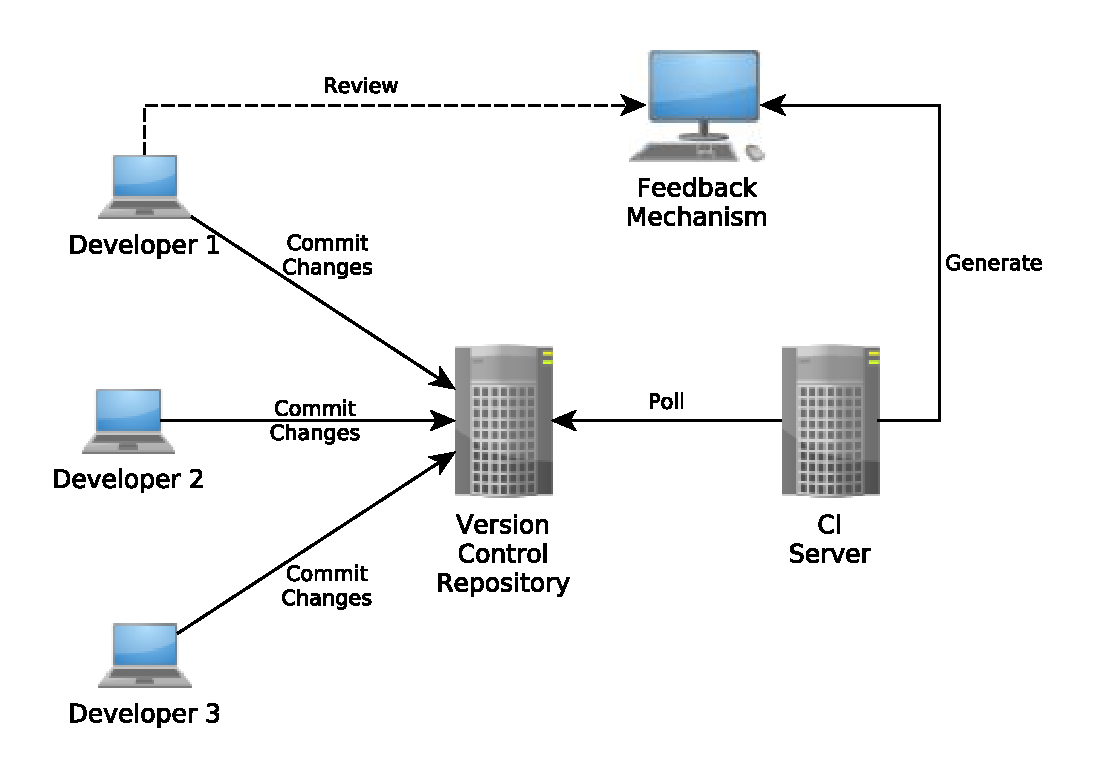
\includegraphics[scale=0.6]{yEd/components_of_CI_system.eps}
    \caption{Components of continuous integration system~\cite{CIbook}.}
    \label{fig:cocis}
\end{figure}

%=====================================================================================
\section{Demands of Continuous Integration}
%=====================================================================================

The minimal requirements for a good software development of a project where multiple developers are working on the same project are a version control repository and a continuous integration server. The version control system guarantees a software configuration management which is required for the continuous integration. The meaning of the version control system is very important. You cannot manage changes that developers had made in the source code without a version control system. The version control system has a very positive impact on the developing project. The system offers a history of changes which may be highly useful if a rollback is desired. Besides the history of changes, this system may save more other information about the source code, e.g. who did the change, when was the change created, etc. In addition, the version control system represents a primary source for the project source codes. This type of project setup is much more often used these days than in the past. Nearly every project has its own version control system which is provided by a repository hosting service.\\

A CI server has a huge advantage. This is a reason why it is highly recommended. It depends on the developer, how does he deploy the CI server. With the CI server, he does not have to bother with such many scripts for the automation. Nevertheless, as he decides how the CI server will be established, the system must contain these features. To facilitate the process of continuous integration, the system must support services as polling version control system, retention of build history, launching predefined steps such as scripts and tests. Furthermore, the system should offer an opportunity to send a feedback back to the developers. This server executes a series of actions or steps taken in order to achieve a particular end of CI. The next section will determine and state these fundamental steps of the continuous integration scenario and describe and illustrate them in detail.

%=====================================================================================
\section{Stages of Continuous Integration}
%=====================================================================================

The stages of CI insure code inspection and code integration. Before we begin, we need to clarify certain concepts which will be used later. To understand these steps, we need to understand what is the difference between \textbf{a build}, \textbf{a private build} and \textbf{an integration build}.

\begin{DEF}
A build may refer to a set of activities performed to generate, test, inspect, and deploy software~\cite{CIbook}.
\end{DEF}

\begin{DEF}
A private build define a process in which a software developer runs the build on his local machine to ensure that the changes he made work before he commits them into a version control repository.
\end{DEF}

\begin{DEF}\label{def:IntegrationBuild}
An integration build is the act of combining software components (programs and files) into a software system~\cite{CIbook}.
\end{DEF}

Figure~\ref{fig:IntegrationBuild} mentions the before stated Definition~\ref{def:IntegrationBuild} which depicts the result of combination individual parts (components) of the software into a single software system. The transformation process that integrate these software components together into a one unified entity is called as an integration build.

\begin{figure}[H]
    \centering
    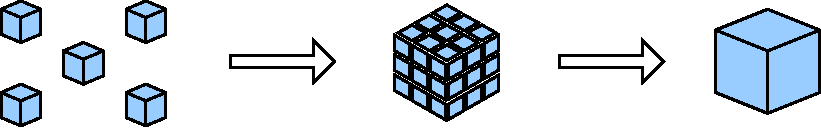
\includegraphics[scale=1]{img/system_integration.pdf}
    \caption{Integration build.}
    \label{fig:IntegrationBuild}
\end{figure}


Now as we know what are these concepts we will illustrate the basic stages of continuous integration. To describe it properly, imagine that we have a group of developers working on the same project using a version control system where the source code of the software product is held, and they use a continuous integration service. The stages of continuous integration are the following:

\begin{enumerate}

    \item \textbf{The change}\\[0.1em]
          One developer who wish to make a change, adjustment, improvement or to create a new feature in the software product has to clone the remote version control repository to his local computer to download the source code of the software product. At this point, he has a local version control repository in which he will do the changes he would like to. After a change is made, the change is only in a local repository and the developer would like to commit it into the remote repository. Before publishing the change, he has to run a private build. The developer has to publish the change he made which is a request for an approval of the change ready to merge into a specific branch on the remote repository. These not merged changes are published on the remote version of the control repository.\\[0.1em]
          By committing changes to the version control repository a continuous integration server is invoked. The continuous integration server polles the version control repository when a change is detected, after this poll a reaction occures.

    \item \textbf{The reaction}\\[0.1em]
          When a change is detected it invokes a continuous integration server to execute a few tasks. The tasks are predefined in a build script which has to integrate the change with the rest of the source code of the software product. The script provide source code compilation, database integration, testing and code inspection. The execution of the script is referred to as an integration build.\\[0.1em]
          This stage of continuous integration usually includes also code verification. It finds defects or errors made by developer, e.g a compilation fail, tests failures etc. The errors are detected by tests which should have high code coverage. A number of errors in this stage can be reduced by launching a private build which may be less complex compared to launching the build script. Passing this stage depends on success of the build script which must be success on 100\%.

    \item \textbf{The feedback}\\[0.1em]
          The continuous integration server generates a feedback associated to the results of the build which is assigned to this change and it might be sent to the author of the change. There is log information generated every time, by passing the reaction stage, and it is held and assigned to the change. Feedback is given to the developer in a certain predefined form, e.g. email with failures only. The log file is saved on the continuous integration server where there is an overview about the builds and their stats.

    \item \textbf{The waiting}\\[0.1em]
          This stage is the end of the process. It stands for continuous polling of  the version control repository waiting for a new change. Detecting a change will cause launching the stages from the beginning.

\end{enumerate}

%=====================================================================================
\section{Continuous Integration Server}
%=====================================================================================

If the software development proceed to use continuous integration in the workflow it might have a configured CI server. The principal sense of a continuous integration server is to get rid of a manual integration build. The configuration of the CI server depends on source code verification requirements and on a type of polling. The CI server can also provide an additional automation for necessary essentials to the development such as integration, deployment, etc.\\

The continuous integration system is based on automation that is conducted by CI server. Automation is an act, when manual tasks are united and executed together in order to simplify the execution of manual tasks. Nowadays, in software development automations can be found in different parts of software development. It helps to accelerate the development process. In a CI system, there are different types of builds and mechanisms used for the automation.

\subsection{Polling}

We can distinguish several types of build mechanisms such as on-demand, scheduled, poll for change and event-driven mechanism~\cite{CIbook}. The simplest automated mechanism, on-demand mechanism, can be done by a single script and it helps to get rid of tasks repetition executed by the developer. The on-demand mechanism is an user-driven process in which someone manually initiates an integration build~\cite{CIbook}. Scheduled mechanism is a planned event accomplished by a CI server in predefined time. In the situation, where multiple developers are frequently working on a product during the day, the best choice for a build should be to plan it in night. The scheduled type is used particularly when an advanced build of the software product is needed to be done. Scheduled processes are driven by time, for instance, so that it runs on an hourly basis, regardless of whether or not a change has occurred~\cite{CIbook}.\\

Poll for change mechanism and event-driven mechanism differ only in a way of invoking. Poll for change mechanism uses a periodic time for a change polling and the event-driven mechanism is time independent mechanism which is invoked by a version control repository. In a poll for change mechanism, a process wakes up in regular intervals and checks for changes to the version control repository, if changes are detected an integration build is ran~\cite{CIbook}. The event-driven mechanism is triggered by the version control repository. If change was detected by the version control repository then it initializes the build script. Only in these two mechanisms, there is a polling service which is sectionalized into two different types.\\

There are two types of polling - time dependent polling and change dependent polling. The CI server with time dependent polling is configured to check the version control repository for a new change in predefined periodic time intervals, e.g., every 10 minutes. Contrawise, the CI server with change dependent polling is invoked with every single action which is a change in a version control repository via an informative message about the current action sent to the CI server. This message including event stats is triggered on a specified event in the version control repository which must support this feature.\\

Time dependent polling is mostly used in general due to inadequacies such as missing event triggering in the version control repository. Due to this fundamental feature some of CI servers has to have  periodic polling on time. The main disadvantage is the time taken by downloading the actual source code from the repository. After the download is complete, the changes are still unknown, and so a comparison must be done between the latest and the last source code for the purpose of obtaining the new changes. Change dependent polling downloads only the real change towards the actual source code status made in the repository. If the version control system can support this feature the source code synchronization is much more faster and efficiently done.

%=====================================================================================
\section{Build Script}\label{build_script}
%=====================================================================================

Instigation of CI system begin with a change in the version control system resulting in build script execution. Transforming sources into a system and simultaneously providing a review about the transformation is an intricate process also known as continuous integration, delivery and deployment. A CI system uses a build script allowing build automation, which includes every predestined statement to execute. This automation had a magnificent impact on software development. To get rid of constantly repeated actions for the purpose to accelerate the software development, a build script was created. The principal script consists of a set of subscripts, which divide the automation into segments that are bound to themselves according to the execution order. Segments are shown in order in Figure~\ref{fig:lpobs}. It shows the logical parts of a build script. Script performs a build also called as a software build which is not just about the source code compilation and tests launch. These various smoothly executed parts construct a functional unit of the software product. A working function unit congregation leads to working software deployment as the final step of CI. The script warrants simplification because of the developers adjust the source code and they are able to gain instant feedback about their work. As Martin Fowler said \uv{Get everything you need into source control get it so that you can build the whole system with a single command.}~\cite{MartinFowler}.

\begin{figure}[H]
    \centering
    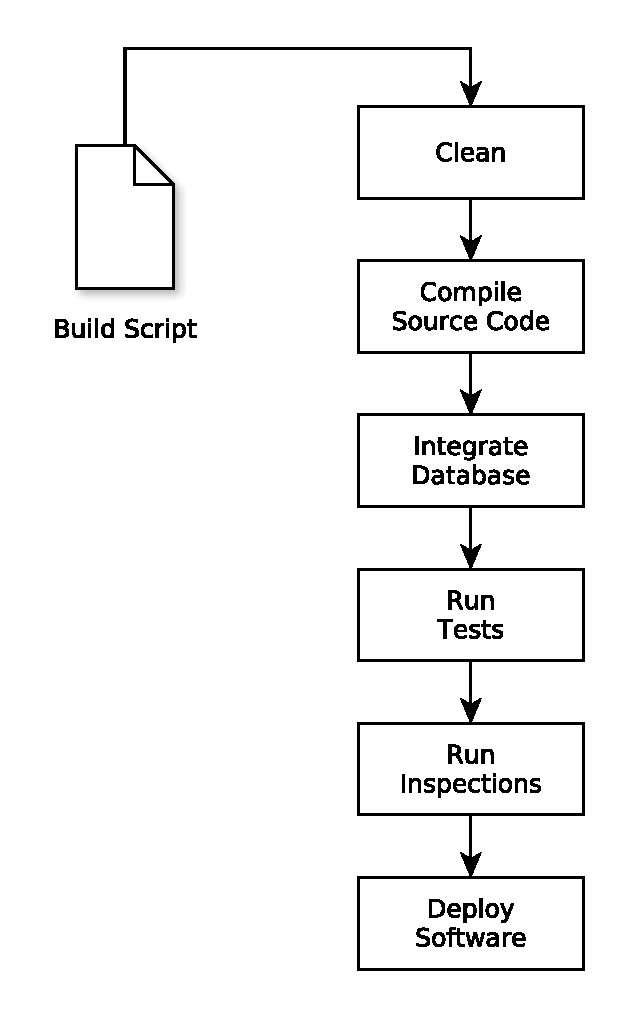
\includegraphics[scale=0.5]{yEd/the_logical_processes_of_a_build_script.eps}
    \caption{The logical processes of a build script~\cite{CIbook}.}
    \label{fig:lpobs}
\end{figure}

The main goal of continuous integration is to provide a rapid feedback~\cite{MartinFowler}. Developers would like to have as fast feedback as possible. To guarantee this quality there are different types of build scripts provided on different kinds of requests. Build scripts are divided by the role as lightweight and heavyweight scripts. Lightweight scripts are much more faster than heavyweight scripts. They are used on principle of speed. To ensure this behavior, at first the lightweight scripts are initiated because they can easily catch the basic vulnerabilities and then more advanced tests, inspections, and others are launched by heavyweight scripts which leads to an integration build. Martin Fowler marked the lightweight script which does the first build, as a \uv{commit build}~\cite{MartinFowler}. These scripts endeavor for quickness, error detection and software integration, besides that, they also provide a feedback about the results of the whole process to the developer.\\

A script is required due to build automation to provide a \uv{press to build} functionality which is executed many times without any interaction. The script has its logical parts shown on Figure~\ref{fig:lpobs}. The transformation process in the first part starts with a clean build, which is nothing more than just clean code compilation. The database integration and the tests execution may be executed differently because of the tests are dependent from the database. Not every test depends on the database, due to this, we can divide them and we may run the database independent earlier then the dependent. If there is an error detectable by database independent than it is caught earlier what is more effective according to the time. After this phase, code inspection is launched for further deficiencies. The last stage of the build script is triggered after every previous stages ended successfully. Outcome of this - is, that the build is an observable result with a log that reflects the build pipeline which forms the basis for the feedback generated for the developers.

%=====================================================================================
\section{Research about the Builds of Continuous Integration}
%=====================================================================================

Continuous integration is a practice, not a tool~\cite{CollabNet}. Martin Fowler on first of May 2006 stated the basics of CI and the best practices of CI in his article in which he remitted on still popularizing usage of CI. In addition to this article, there was a research provided by a group of scientists about the CI on a project provided for the most part from GitHub. Their research is an empirical study about the usage, costs and benefits of CI which are concisely shown in abundant diagrams. The observation of CI and its usage pointed out the significant essential role of CI in open source projects. On the basis of the informations obtained from the researches about the CI, we can make a judgment that this practice will be more and more used in the open source projects. Thanks to automation and standardization, CI helps to effectively prevent errors when deploying applications into operation~\cite{CIcure}.\\

Continuous Integration is also referred to as a \uv{cure for human error in deployment}~\cite{CIcure} because of error prevention which is rapidly reduced by using this practice. The job of a developer includes a project build repetition which may be also reduced in the sense of tasks rate reduction applied on developer. These processes leverage extensive automation and encourage constant code sharing to fix defects early~\cite{DigitalOceanCI}. Many of errors, bugs, defects and vulnerabilities are reduced but not every of them is detected by using a CI, but nevertheless the manual software integration is excluded because of CI comprises it as the last step of the software deployment. The impact of the CI usage in software engineering will have extreme influence on the future of IT, more precisely in agile teams using extreme programming technique or any other agile technique. The usage of CI is very adaptive and versatile and it will be more and more used in forthcoming open source projects or any another projects which may not be open source only.\\

In general, if any group of developers would like to use a CI practice, they should fulfill few standards and take heed to these standards. In order for developers to benefit from use CI in practice, they should change their typical day-to-day software development habits~\cite{CIQualityFramework}. Usage of CI is a beneficial sideline when a developer commits frequently, daily, often, probably few times per day. Farthest, the project should be hosted somewhere on any kind of version control repository which represents a main source for the source code of the product. Besides these two sole development requirements, the expectations are that the developers should not try to commit a broken code. It is avoidable by initiating a private build on their local machine, which decreases the fail chance of the build launched by the CI server.\\

By using CI practice, the risks as software corruption and integration problems are reduced appreciably and any kind of bugs are uncovered quickly. The integration may take unpredictable long time but the use of the CI practice resolve this problem by integrating the software frequently which may result in a few small kind of integration issues. Some other software methodologies integrate their work once after a long time which brings their software to face an incredibly huge integration problem. Martin Fowler pointed this problem in his article: \uv{I was told that this project had been in development for a couple of years and was currently integrating, and had been integrating for several months.}~\cite{MartinFowler}. Several articles describe this long time integration as a \textit{Big Bang Integration}~\cite{AaltoUniversity}. As we can see on Figure~\ref{fig:integration} the risk of the software integration is markedly reduced by using a daily (continuous) integration which is used in a CI practice.

\begin{figure}[H]
    \centering
    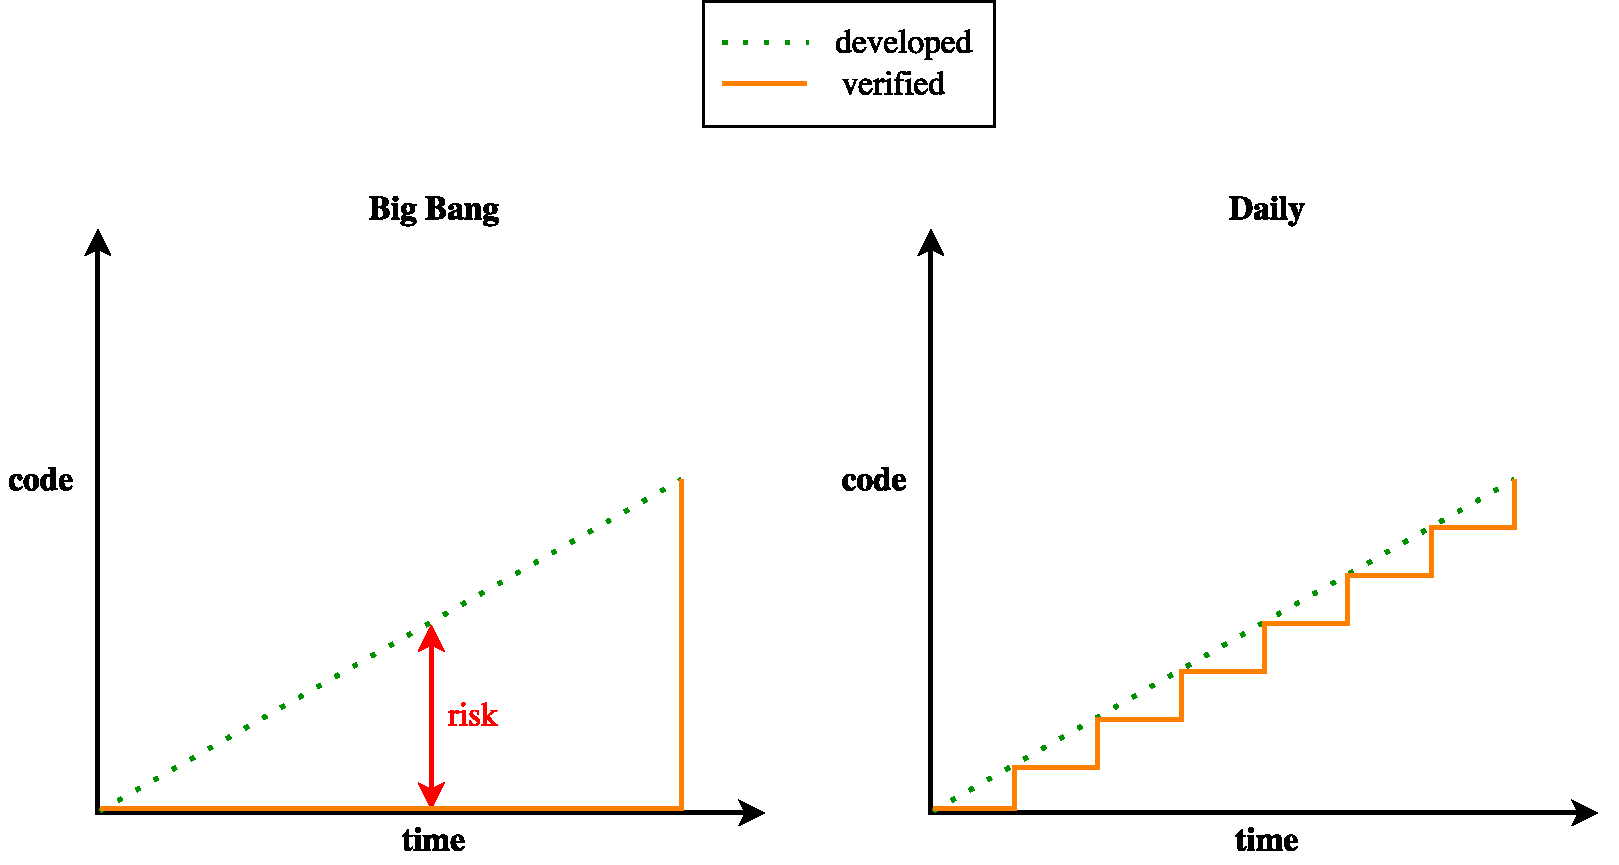
\includegraphics[scale=0.5]{img/big_bang_vs_daily_build.pdf}
    \caption{Comparison of integration builds~\cite{AaltoUniversity}.}
    \label{fig:integration}
\end{figure}

\begin{displayquote}
    \textit{\uv{Not integrating continuously is expensive. If you don’t follow a continuous approach, you’ll have longer periods between integrations. This makes it exponentially more difficult to find and fix problems. Such integration problems can easily knock a project off-schedule, or cause it to fail altogether.}}\\[-2em]
    \begin{flushright}
        -- ThoughtWorks$^{\tiny{\textregistered}}$~\cite{ThoughtWorks}
    \end{flushright}
\end{displayquote}

Prevention against any type of error in a CI is solved via integration build performed on a CI server. Predicting the result of build has drawn the interest of academia and industry~\cite{ResultsOfCIbuild}. In term of build result analysis and prediction, most existing studies focused mainly on a large software project developed and maintained by big companies~\cite{ResultsOfCIbuild}. Travis CI community has created a TravisTorrent\footnote{The name of TravisTorrent was chosen to resemble the close proximity to the GHTorrent project~\cite{TravisTorrentWEBPAGE}.}~\cite{TravisTorrent} for the purpose of providing a huge amount of information about the builds for full-stack research on continuous integration which is still a developed prototype. Alongside the TravisTorrent, the GitHub company has provided information about the data inside of their version control system in a project called \uv{The GHTorrent project}\footnote{The name signifies a torrent of data coming from GitHub~\cite{GHTorrentWEBPAGE}.}~\cite{GHTorrent}. Based on these given informations as an open dataset, a few analysis were conducted on them resolving the CI practice in a real life developed projects. The best practices were established on the results of the empirical studies of these obtained data sets provided by many of associations.\\

Studies about the CI were facing against difficult analysis due to inaccessibility of the project's data such as projects of private companies. Due to this, the observations are related to projects mainly hosted on GitHub and predominantly using Travis CI. Informations received from these observations are impressive and they point to the popularizing usage of the CI or promoting CI adoption in projects nowadays. Continuous integration is emerging as one of the biggest success stories in automated software engineering~\cite{COPE}.\\

The most interesting question is that how many projects are using the CI at all? In year 2016, an empirical study stated 40\%~\cite{COPE} of the projects, observed by them, are using CI practice. Despite of this result, they noted that the number is still growing and it will be still growing more intensively. While CI is widely used in practice nowadays, we predict that in the future, CI adoption rates will increase even further~\cite{COPE}. The results are shown in the Table~\ref{table:CI_usage}.

\begin{table}[H]
    \centering
    \begin{tabular}{lrr}
        \hline
        Projects Uses CI? & Percentage & Number of Projects \\
        \hline
        Yes               & 40.27\%    & 13,910             \\
        No                & 59.37\%    & 20,634             \\
        \hline
    \end{tabular}
    \caption{Usage of CI in projects~\cite{COPE}.}
    \label{table:CI_usage}
\end{table}

The adoption of the CI to the project may depend on many factors which include, for example, familiarity developers with the CI which is the main factor. The median time for CI adoption is one year~\cite{COPE}. The basic reason of putting the CI into the development is due to bugs and error reduction, but there is still a possibility of a bug or error incursion into production. As Martin Folwer said \uv{Continuous Integrations does not get rid of bugs, but it does make them dramatically easier to find and remove.}~\cite{MartinFowler}.

%=====================================================================================
\section{Best Practices of Continuous Integration}
%=====================================================================================

The continuous integration practice has become very exploited and its usage has increased considerably the overall agility and efficiency in the development process. It helps stakeholders, testers and product owners to work together seamlessly eliminating bottlenecks and achieve faster time to market~\cite{CI-BP1}. This section describes fundamental practices which can lead to dramatical decrease of the costs on the project by using this approach to the CI practices. The costs reduction may be approximately 40\% less as the Ade Miller's study~\cite{100DaysOfCI} has shown. The influence may be avowedly known while using these practices. The effort of maintaining the CI system and the usage of the fundamental practices for CI has a magnificent impact on the project. Project investment into a CI usually leads to costs reduction, agility growth and error reduction in the development process. Some of the scientific studies report a different number of the CI practices but the general idea of these practices is same in each of them. Studies investigate more likely GitHub projects due to the free available informations, from GitHub projects in the GHTorrent and TravisTorrent projects, and on this basis they established these practices.

\subsection{Maintain a Central Code Repository}

As a fundamental requirement for the CI is a version control system where a principal repository is held. Software development project involves multiple developers constantly working and pushing code files that need to be orchestrated together to build a product~\cite{CI-BP1}. Maintaining a system like this includes a lot of advantages as a source code backup, a reference on the primary mainline of the code with the latest content and a much more others. However, it is mainly used as a source for latest and clean source code of the developed project. This is a basic part of the setup for every project developed by a group of people who would like to share a code in the most common way in the development life. Nowadays, it is a often used practice nearly for everybody working on some software product in the development and alongside CI practice is necessarily used.

\subsection{Commit Code Frequently}

The continuous integration approach requires to commit at least once per day into the baseline. The CI is based on frequent integrations where the integration is initialized by a new commit. The fact that the commit starts the whole process which may be halted at testing part not necessitate but recommend to update the local copy of the mainline to resolve possible conflicts which may halt the process too. After the update, the newly added changes are ready to be checked by a local build which prevent the fail of testing part of integration. The daily commits will result in frequent integrations that keep the mainline in stable state and good condition. Because of there are many commits, one rule applies to them which should be kept. A commit should have a characteristic attribute of atomicity which divides the code in two parts as before adjustment and after adjustment. It means, that the commit forms a logically comprehensive unit of changes. The frequent commits better the collaboration because of source code sharing between developers and oftentimes run an integration builds of the mainline on the integration machine that checks the mainline status.

\subsection{Do Not Commit a Broken Code}

Broken code is a code that contains any type of failure when it is included in a CI build~\cite{CIQualityFramework}. As a prevention against committing a broken code to the shared code repository there is an opportunity to run a private build on a developer's machine before each commit. A private build detects the simplest mistakes such as a syntactic error or any other error forgotten in the code which are easy to detect. To reduce the plain error inside of the committing code, developer may use a code linter, if a developer uses an IDE\footnote{Integrated Development Environment}, it may has a build in linter. Code linting is a process of running a program which provides a code analysis for potential errors. Some of these basic errors are not detected by the linter so this is the reason why a developer should launch a private build before every single change he would like to commit. A private build may include a simple test set to detect these potential errors and defects in a created change. To commit a non broken code stands for to run a private build on a developer's local machine before committing his changes. This circumvention may accelerate the change integration.

\subsection{Fix Broken Builds Immediately}

An error consequences may beget a broken build as a result of the CI failure. Outcome of this action is an feedback which is sent to the developer as a fix requisition. Developer responsible for this problem should fix it as fast as possible irrespective of the build time cost. Fixing a broken build should be the top priority of the project~\cite{CIQualityFramework}. As Martin Fowler quoted Kent Beck in his article \uv{Nobody has a higher priority task than fixing the build.}~\cite{MartinFowler}. The meaning of this build fixing is not to stop the actual tasks given to the developers, instead of this, it means to get couple of versed project members to fix the build. CI is effective while the build of the mainline, the principal branch of the project, has a successful termination result. Keeping an operational code in the repository forms the basis of CI which signifies a development on a stable based code. Effectiveness of the CI, while the code is stopped at build and not progressing to the integration into the software product, is low. To keep a mainline without broken build is almost always an unfeasible or nearly impossible task due to the human factor. The core idea of this part, how to ensure a mainline without broken builds, is to prioritize the urgent fixes and realize them if needed.\\

Some of the build fix solutions involve dropping the last commit - last change reversion. To avoid broken builds and enhance the solution mentioned before a new practice has been introduced - the pending head. Usage of pending head is a prevention for broken builds of the mainline. A pending head is a way how to indirectly commit a change into the mainline for the reason of a build make. The result success of the build decides about passing the commit into the mainline.

\subsection{Keep the Build Fast}

The stumbling block of the CI practice is the duration time of build. Because the build and test steps must be performed frequently, it is essential that these processes are streamlined to minimize the time spent on these steps~\cite{DigitalOceanCI}. Build time may be inappropriately long, which is unacceptable for the developers and can lead to the disfunction of CI. Every minute you reduce off the build time is a minute saved for each developer every time they commit~\cite{MartinFowler}. The most crucial and meaningful solution for reduction of the build duration is to use inside of the build a pipeline. Build is executed by a build script which can be divided into parts which were described in Section~\ref{build_script}. According to the reduction of the build time, tests take a long enough part of the build time too. A CI practice laboriously relies on the unit test which runs approximately equal to core components which makes them very fast. They are the first line of defense in ensuring quality~\cite{CI_atlassian}. Vice versa, the API\footnote{Application programming interface} and functional tests are greater time consumers due to their complexity. Graph in Figure~\ref{fig:grap_dependence} depicts the dependence of these two factors. A solution of this situation lies in a well chosen pipeline of the deployment, more  precisely, how to run multiple builds in phases properly. When possible, running different sections of the test suite in parallel can help to move the build through the pipeline faster~\cite{DigitalOceanCI}. A useful consideration of using many of unit tests with high code coverage which have minimal maintenance may also lead the build to time reduction.

\begin{figure}[H]
    \centering
    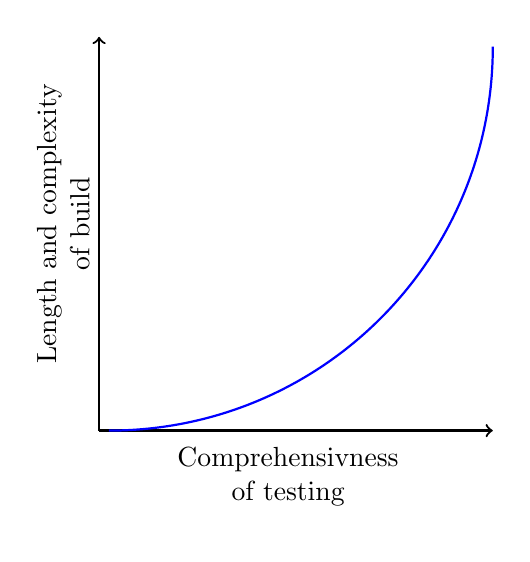
\begin{tikzpicture}[scale=0.5]
        \node[] (i) at (0, 0) {};
        \node[] (l) at (10, 10) {};

        \node[label={[align=center,rotate=90]Length and complexity\\of build}] (left_text) at (0, 5) {};
        \node[label={[align=center]Comprehensivness\\of testing}] (right_text) at (4.8, -2.4) {};

        \draw[draw=black, thick, <-] (10, 0) -- (0, 0);
        \draw[draw=black, thick, ->] (0, 0) -- (0, 10);
        \draw[draw=blue,  thick] (i) to[out=0, in=270] (l);
    \end{tikzpicture}
    \caption{Dependence between length and complexity of the build and comprehensiveness of tests~\cite{deployment_automation}.}
    \label{fig:grap_dependence}
\end{figure}

\subsection{Everyone Can See What Is Happening}

Continuous Integration is all about communication~\cite{MartinFowler}. Using a CI practice means to share all the gathered informations with the project members. Anybody from the team members should see the informations about the adjustment in the code that somebody had created. But it is not just about others work it is about the project state and the changes which have been made inside of it and about the new ones which will be integrated into it.\\

The fundamental part of the CI is the granted feedback about the result of the build realized by the CI server. Feedback is a summary of the log generated during build. These informations about the build status should be easy to obtain for anybody ensuring the development speed and quality. Developers must know the status of their adjustment after being handed over to the build. The news in the feedback are very important, especially at some build break. Information obtained from the feedback serves to fine-tune the made adjustment by the creator. Every single build result is assigned to the belonging commit (adjustment) which was made. These informations should be retained for the case if somebody would like to look at a build passing in the past - build passing before the current state. Developers should easily gain these informations and they should be notified if any kind of build broke arises on their work.

\subsection{Automate Deployment}

Automating deployment helps to reduce waste~\cite{CollabNet}. Automated deployment is nearly adherent to release automation. An essential part of releasing a software product is deploying it, first on development environments, then on QA\footnote{Quality Assurance} and UAT\footnote{User Acceptance Testing} environments, and finally on the real production environment, either on the developing organization's premises, on a customer's premises or on the cloud~\cite{deployment_automation}. The usage of the CI required multiple development environments. Consequently, that you have to move the binaries between multiple environments which follows to create scripts if no manual work is wanted. This allows to deploy application across various heterogeneous environments used in the development process including the final production environment automatedly. In these days, there is an interest in virtualization which allows to create the expected environments easy and simple by putting together these virtualized environments.\\

If the application meets all standards and criteria it is deployable. You have to pay special attention to the deployment. There always was, is and still will be a chance of a failure, due to this fact a failure of application deployment requires a rollback. This rollback provides a certain decrease of difficulties about the deployment. Automated deployment, tied into good CI discipline, is essential to make this work~\cite{MartinFowler}.

%=====================================================================================
%=====================================================================================
\chapter{Automated Code Review}
%=====================================================================================
%=====================================================================================

Development has adopted code review practice a long time ago. As software engineers collaboratively develop software, they need to understand, analyze, and validate past and present program modifications made by other developers in order to detect inconsistent, potential defects, manage the impact of the changes on structural anti-patterns, and avoid validation failures due to the lack of test coverage~\cite{CodeReview_bug_and_refactor}. Nowadays, it is an ordinary well-known practice which influences the overall code quality. Reviewing the source code is a complement to other quality mechanisms, such as compiling, integrating and testing~\cite{CodeReview_types}. This practice rests in idea of revising others work by others which points to collaboration on the same code by multiple people, especially co-workers. Today, this practice has been influenced by a lot of development practices and habits which lead to the use of code review in a development progress. An idea has arisen to automate this process which should speed it up due to its time costs. The practice has been successfully automated but it is not fine-tuned already. There are many suggestions how to improve the code review quality and speed which cause code review more effective. The next sections describe code review, its types and how it is deployed in today's software development.

%=====================================================================================
\section{Code Review}
%=====================================================================================

Code review is a substantial part of the development which improves the source code quality markedly. The importance of the code review lies in the code enhancement that is significant towards not reviewed code. Code quality is made by imperfection reduction. Analysis of the code by someone else than the author who has a different type of view on the code may result in an imperfection detection. The reviewer, who is not the author of the code, can be a person or a software. This reviewer type division involves two types of code reviewing - the automated code review and the non automated review which is done by a developer. Human is irreplaceable by a machine but machines do not make mistakes. This is the reason why the development process includes both types of code review. Automated code review functionality is supported in many of IDEs which informs the developer about the vulnerability in real time. This feature may involve static code analyzing tools which provide an extremely fast feedback. Rigby and Bird (2013) find that current software inspection practices tend to converge on Modern Code Review (MCR)~\cite{review_participation}. The non automated code review also known as manual code review is done by a person via some code review tool. The person is usually a project member who has to known at least the fundamentals about the code which he has to review. Review ends with a code criticism which should be taken by an author positively because of it enhances his code not degrades it. Software code review is a well-established software quality practice~\cite{review_participation}. Code review can improve the quality of software products by identifying weaknesses in changes early in the development cycle (Fagan 1999; Shull et al. 2002)~\cite{review_participation}.

%=====================================================================================
\section{Principle of Code Review}\label{fig:sec_pri_CR}
%=====================================================================================

The resulting work of a person normally involves deficiencies and faults because of the imperfection of people. The amount of imperfections depends on the skills and the experiences of an individual but they are still not removed completely. To catch the rests of non-caught vulnerabilities require to examine the work, the source code in case of development, by collaborators or project members. The examination of the work result is called in the development as a code review. To understand what is a code review or source code review there are different type of definitions.

\begin{DEF}
Source code review is an act of consciously examining source code intended to find bugs at an early stage of software development~\cite{CodeReview_eye_tracking}.
\end{DEF}

\begin{DEF}
Source code review is an offline task aimed at finding the bugs in a code without compiling or executing the code~\cite{CodeReview_eye_tracking}.
\end{DEF}

Usage of this practice is reflected on the quality of the source code which is rationally premeditated due to different types of reviewers view. Code review explicitly addresses the quality of contributions before they are integrated into project's code base~\cite{CodeReview_quality}. A research article stated that a large portion of faults has been found by only one reviewer~\cite{CodeReview_evaluation}. As many of reviewers are participate on a review, many deficiencies of the code are annihilated.

\begin{figure}[H]
    \centering
    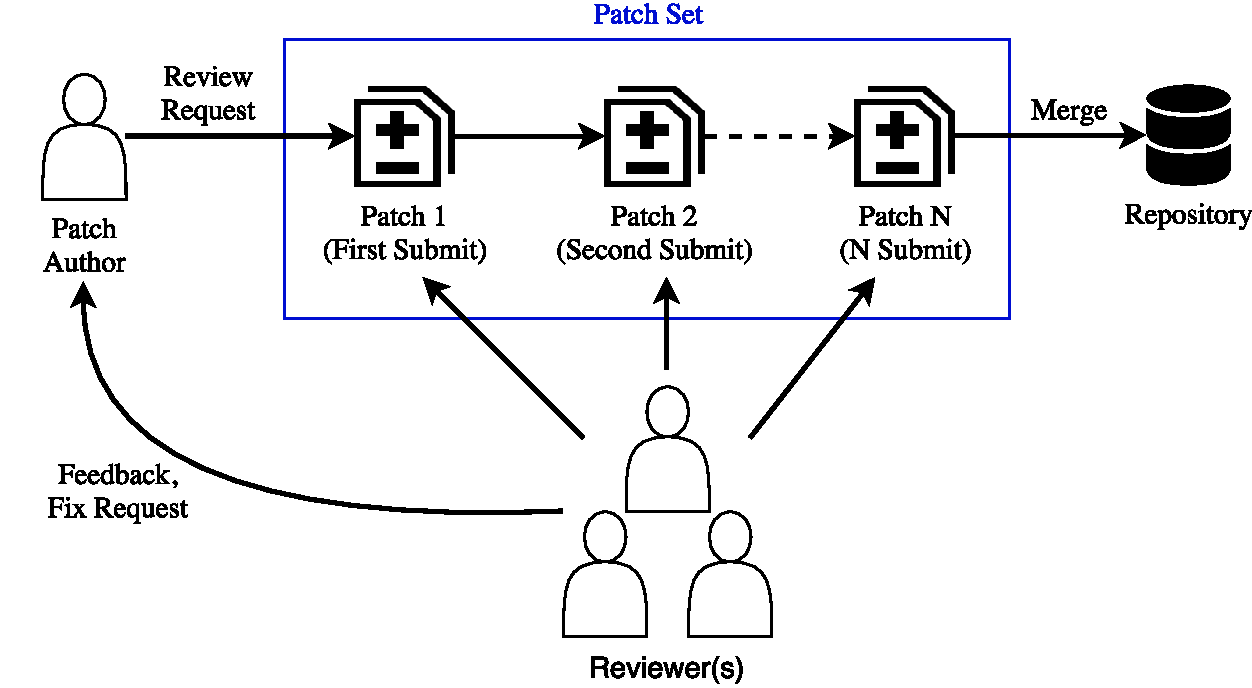
\includegraphics[scale=0.5]{img/process_of_review.pdf}
    \caption{Code review process~\cite{CodeReview_IFstatement}.}
    \label{fig:review_process}
\end{figure}

Code review always starts with a request for a review of some patch which is a modification of the actual source code. This patch is reviewed by somebody who has knowledge about this field or it is related to his field. The reviewer may approve this patch which leads to a merge of the patch into the actual source code in the repository - the project code base, or he may request for a fix from the author. This request for a fix does not mean that the patch is impaired, it will enhance the patch instead of patch degradation. After a fix request, the process is repeated until an approval. This process in non-automated, also called manual, because it is done by a person or a group of people. In an agile development, a thought has arisen which tried to automate this process. The impact of continuous integration on code review process is not yet properly understood given that they are interleaving steps in the software quality management~\cite{CodeReview_impact_of_CI}.

%=====================================================================================
\section{Types of Code Review}
%=====================================================================================

There are many of code review types depending on the aspect, view and the review provider. Code review is divided into two basic types such as manual or automated. The reason of this division rests in the reviewer type. The reviewer may be a person who has to review the whole code or a software which processes the code according to the predefined set of rules.\\

The manual code review is a code examination of others work provided by a person. This type of review was described in Section~\ref{fig:sec_pri_CR} and shown in Figure~\ref{fig:review_process} what constitutes the basis of this practice. The difference from automated code review is the fact, that the manual code review includes a human person who has to give the review judgment - the approval or a request for a change.\\

To automate this practice, it is necessary to have a definition of project-specific rules. The automated code review is based on a predefined set of rules and best practices which are checked by a software whether the conditions are met or not. Matching these rules is provided via software which includes static analysis tools for this operation. As manual code review includes at least one person, the automated code review includes a static analysis tool which represents the person and performs his job in the code review. Static analysis tools for automated code review are the most effective~\cite{CodeReview_security}. This automation is only refinement of manual code review due to its duration.\\

Nowadays developments usually use both approaches. The major purpose is to catch as many deficiencies as possible to reduce the insufficiency of the software product and increase its overall quality. Manual review is such a pain that reviewers regularly suffer from the \uv{get done, go home} phenomenon - starting strong and ending with a sputter~\cite{CodeReview_security}. This factor may be circumvented with automated code review but it has its deficiency too because it is limited by the number of rules. It cannot catch defects which are not defined the set of rules. These two fundamental reasons lead the development to adopt both types of code review.

%=====================================================================================
\section{Automated Code Review}
%=====================================================================================

Automation cannot be achieved without any static analysis tool. A static analysis tool is included in a software which provides a static analysis which is performed without any compilation or any execution of the analyzed source code. Static code analysis finds a wide range of issues such as code style, code best practices, security, complexity, compatibility etc~\cite{codacy}. The terminology includes an expression defined for a static code analysis which is named as a code inspection. The software which provides the static analysis of the source code with the adequate tool mentioned before is called as a linter. Also the usage of this software has created a notion \uv{linting} which is a process of running this software that analyses the source code. There are many linter types which variety depends on the language of the source code it has to analyses for the deficiencies. These widgets are often used in a CI practice due to error uncover before applying the modification and adjustments into the source code.\\

Automated code review is a process in which a software checks the source code for compliance and observance predefined via rules and for insufficiencies which could lead to potential errors. These rules represent a specific patterns which have to be adhered. Keeping the rules leads to better code quality and orientation of developers in the code due to one coding style which was chosen to be abode. This type of code review is an analytical solution for code checking which does not include source code compilation. The result of this process involves a list of violations and contravention of standards and principles which have not been complied with. The source code after solving these detected inaccuracies is faultless and without any potential error and also in one coding style. Due to the fact that this type of code review forces developers to use only one approach to coding guideline which helps to make the code readability much more better unlike mixing multiple coding styles together as a result of collaboration. In agile software development with manual code review, this practice has a considerable demand on the review speed in the development process. Because of this, oftentimes the development chooses a selection of both review types usage in the development considering that these types complement each other. Nowadays, there are plenty of these application providing static code analysis which have their utilization nearly in every project.

%=====================================================================================
\section{Automated Code Review in Continuous Integration}
%=====================================================================================

This type of code review is oftentimes used besides a CI practice in which it has an appreciable impact. Many times the detected offenses break a build initialization in a CI pipeline. The build is useless if any of critical defect is included in the source code because of the time costs of the process which will even thought find this defect. Automated code review is fast enough to be used beforehand build initialization to decrease a chance of worthless build execution. Besides the usefulness of automated compilation and testing software projects can greatly benefit of the execution of automated static code analysis tools within CI~\cite{SCA_in_CI}.\\

% TODO REMOVE
\begin{comment}
My Notes:
 - https://web.archive.org/web/20110927010304/http://www.ida.liu.se/~TDDC90/papers/industrial95.pdf
 - http://ieeexplore.ieee.org/document/7962383/
\end{comment}

%=====================================================================================
%=====================================================================================
\chapter{Implementation}\label{chapter:implementation}
%=====================================================================================
%=====================================================================================

The fundamentals of the implementation part of this thesis were established on deficiencies and issues related to the ManageIQ Bot~\cite{MIQBOT}. A list of missing needs of the bot were created by the developers and more important of them were chosen to be implemented. The goal of the tasks was to reduce these deficiencies and issues by implementing and adding them into the currently working bot. Besides of the implementations of bot's missing features there were a plenty of problems and issues as a side effect which had to be resolved as fast as possible. The implementations of the bot's missing needs were added via pull request to the ManageIQ Bot repository which had to be checked before merging by the maintainers of the repository. The pull request checking - the pull request review, was a little bit slowly because of the maintainer's busyness. The result of these features may help developers with a little increase of the team agility and simplifying some of their needs targeted on the bot. I hope and believe that these added features will help developers in their daily work. Some of the features are added already, but some of them are still not added yet because they are waiting for their pull request merge or approval.

%=====================================================================================
\section{ManageIQ Bot}
%=====================================================================================

The ManageIQ bot is the ManageIQ team's helper to automate various developer problems~\cite{MIQBOT}. The automation of these manually provided tasks by developers increased the team agility because of time saving for major tasks. In addition, this bot reacts on specific commands used by the project members on which he performs a desired action. The bot's core is based on Sidekiq\footnote{\url{https://github.com/mperham/sidekiq}} which is a simple background processing for ruby. Due to the fact that the bot is not using GitHub's Webhooks\footnote{\url{https://developer.github.com/webhooks}} he is configured to use a polling method instead. The polling method rests in a specific content downloading repetitively via GitHub's REST API v3\footnote{\url{https://developer.github.com/v3}} over HTTPS. The downloaded content contains JSON data from which are the necessary informations extracted and on their basis an action or multiple actions are performed. Some of the bot's actions results in a GitHub actions such as posting a comment, adding a label or milestone that are using HTTP requests via the mentioned REST API v3. These actions are used to facilitate the manual tasks resulting in a complete elimination of them from the developer's tasks.

%=====================================================================================
\section{Pronto}
%=====================================================================================

Pronto is a tool that provides an automated code review of new changes in a git branch~\cite{PRONTO-1}. It is typically used in continuous integration as a way to provide feedback on a pull/merge request~\cite{PRONTO-1}.\\

The Pronto~\cite{GITHUB-PRONTO} integration was necessary due to the unification of the output of multiple static code review services. Pronto provides a quick automated code review by analysis of the relevant changes with the related static analysis tool to the source code. The main advantage is that it has its own formatters which are very useful. If the output is desired to be formatted for GitHub, BitBucket, GitLab or any other supported format than the built in formatter provide this expected feature. The format type - pull request, pull request review, etc., is also supported. The result of formatters is configurable via configuration file which defines the desired format of the produced message. Henceforth, Pronto is able to run multiple different static code analyzing tools such as RuboCop, YAML-Lint, HAML-Lint, etc., which are united under Pronto. They are united because of only one output is expected with a summary of the analysis results.\\

To unite these various tools, Pronto had encapsulated every single tool into a Pronto plugin - a Pronto runner. This runner represents a middle layer between the Pronto application and the tool - the static code analyzing tool. The encapsulation facilitates the unification of these tools at the end of the source code analysis process. The Pronto runner provides an automated code review for a specific programming language by the corresponding linter. This linter union was a great simplification of running all expected linters together.

\subsection{Issues}

During the integration process, a few problems were discovered which had to be resolved. The main issue of this integration was a pattern matching of the Pronto output with the original output of the code reviewing part. This integration required to create exactly the same data structure from the Pronto result as the original data structure was because of further usage in the bot - compatibility with the original structure of the results. Furthermore, a bug has been found during the testing of Pronto. A Pronto runner does not include an offense about a syntax error. This type of offense was detected by linter but the encapsulation of this linter into the runner caused that this offense was threw away.

\subsection{Integration}

The integration process of Pronto involves implementation of Pronto result converter, unit tests, bug fixes and enhancements with some of them being designed after review of the pull request\footnote{\url{https://github.com/ManageIQ/miq_bot/pull/406}} by the developers. To integrate Pronto without changing the original behavior of the bot required to launch Pronto with the authentic linters and convert the Pronto result to match the original data structure pattern of the offenses. Before the Pronto analysis a temporary folder is created where the examined repository is copied whose content is located in a subdirectory \textit{repos} of the bot. After that, a repository object is created based on the actual temporary folder content which is fetched. The last stage of this part rests in gathering the patches which are passed to the Pronto runners. The execution of Pronto runners results in the expected output - an array of pronto-message objects. An one object which has type of pronto-message contains every information about one patch of line including the linter result describing this line. An example of a single pronto-message is shown in Figure~\ref{fig:pronto_message}.

\begin{figure}[H]
\begin{lstlisting}[basicstyle=\scriptsize, xleftmargin=.21\textwidth]
#<Pronto::Message:0x000056452d8dcef8
 @commit_sha="1d4e09dc52421b8adeab39f37728aca95a4fc462",
 @level=:warning,
 @line=
  #<struct Pronto::Git::Line
   line=
    #<Rugged::Diff::Line:47427558500720
    {line_origin: :addition, content: "puts 'Hello' \n">,
   patch=
    #<struct Pronto::Git::Patch
     patch=#<Rugged::Patch:47427542553580>,
     repo=
      #<Pronto::Git::Repository:0x000056452b969698
       @repo=
        #<Rugged::Repository:47427542010600
        {path: "/tmp/d20180323-13013-1lkcejq/.git/"}>>>,
   hunk=
    #<Rugged::Diff::Hunk:47427558501220
    {header: "@@ -0,0 +1 @@\n", count: 1}>>,
 @msg="Layout/TrailingWhitespace: Trailing whitespace detected.",
 @path="space.rb",
 @runner=Pronto::Rubocop>
\end{lstlisting}
\hfill\\[-3em]
\caption{Example of Pronto::Message object.}
\label{fig:pronto_message}
\end{figure}

After obtaining the pronto result in a form of an array of pronto-message objects the creation of the identical data structure which has to match the pattern of the original data structure can begin. Originally the linters were run sequentially while their results were appended into an array which is shown in Figure~\ref{fig:run_all_linters}. The result was a data structure including structures about the detected offenses belonging to the specific files sorted by linters. This type of liters lauching is via Pronto much more easier because of the developers have to specify only the gem in the gemfile and there is no need to change a large amount of source code. A Gemfile describes the gem dependencies required to execute associated Ruby code~\cite{Gemfile}. Expected linters have to be specified only in a gemfile by using the corresponding gems for the Pronto runners responsible for the linters.

\begin{figure}[H]
\begin{lstlisting}[basicstyle=\scriptsize, xleftmargin=.27\textwidth]
unmerged_results = []
unmerged_results << Linter::Rubocop.new(branch).run
unmerged_results << Linter::Haml.new(branch).run
unmerged_results << Linter::Yaml.new(branch).run
unmerged_results.tap(&:compact!)
\end{lstlisting}
\hfill\\[-3em]
\caption{Example of linters launch.}
\label{fig:run_all_linters}
\end{figure}

The example shown in Figure~\ref{fig:run_all_linters} is a function body which was completely replaced. In order to maintain the same functionality, a converter was created which replaced this function body. This changed function works on the principle of retrieving the pronto result which is converted to the same structure as the original was. The pronto result is obtained via a function which creates a temporary folder in which the branch content is copied, fetched, analyzed and the patches describing the changes are passed to the pronto which runs the pronto runners resulting in an array of pronto-messages. This array is iterated over and its content of pronto-message objects from which are the necessary informations extracted, is mapped to the structure describing the original one. The informations describing the linter and the platform were not added to the results as it originally was because they were not applicable. The method of linters launching shown in Figure~\ref{fig:run_all_linters} was completely redesigned and simplified. The result of pronto integration is a linter unification that guarantees triggering of different linters which have to be specified only in the gemfile.\\

Except the pronto integration, a bug was detected and it had to be fixed via a pull request\footnote{\url{https://github.com/prontolabs/pronto-rubocop/pull/35}} into the pronto runner for RuboCop. After code analysis by this RuboCop runner, the runner does not return a detected offense in the source code describing the syntactical error. The syntactical error was detected by the RuboCop as an offense, see Figure~\ref{fig:syntax_offense}, but it was not mapped to the final result of its runner.

\begin{figure}[H]
\begin{lstlisting}[basicstyle=\scriptsize, xleftmargin=.14\textwidth]
#<RuboCop::Cop::Offense:0x00007fc750319218
 @cop_name="Lint/Syntax",
 @location=
  #<Parser::Source::Range /tmp/d20180324-16231-1bppist/syntax.rb 101...101>,
 @message=
  "Lint/Syntax: unexpected token $end\n(Using Ruby 2.3 parser; confi" \
  "gure using `TargetRubyVersion` parameter, under `AllCops`)",
 @severity=#<RuboCop::Cop::Severity:0x00007fc7503191f0 @name=:error>,
 @status=:unsupported>
\end{lstlisting}  
\hfill\\[-3em]
\caption{Example of offense related to syntactical error.}
\label{fig:syntax_offense}
\end{figure}

% BUG
\begin{comment}
Command `make normostrany` fails here (the lstlisting above). The ruby code above contains $ which stops the `detex -n FILE` at this point and the text behind the $ is ignored until the end of this file.
\end{comment}

The fact that the error is not reflected in the result was solved via additional inspection of the offenses. Firstly, the offenses are selected by the patch line where the line number of the added patch is matched with the line number of the offense. If they match then the offense is selected. This was the reason why the Pronto runner for RuboCop dropped the offense about the syntactical error. At selection the number of the offense line was excluded in the line numbers of the patch. Due to a syntactical error, the offense's line number was a number given by a ruby parser which was not adequate to the number of added lines in the patch. These offenses are added additionally at checking the offenses secondly looking only for the syntactical errors. If there is any syntactical offense, it is detected in the second phase of offense mapping by the cop name which includes information about the syntax error, and it is added to the result as an offense detected on the last patch line.

\subsection{Enhancements}

By using an automated build practice as an part of continuous information approach, the added source code must have its unit tests. The unit tests had been replaced with the newer one covering the actual source code which is added. The unit tests are checking the conversion from an array of pronto-messages to a data structure describing the offenses which was originally used. Some of the informations such as a ruby platform, a ruby version, a ruby engine, etc. were not used from this data structure and they were removed. Moreover, due to the wicked results of the offenses because of infringed convention for naming pronto runners the relative runner was fixed\footnote{\url{https://github.com/pauliusm/pronto-yamllint/pull/2}}.\\

After submitting changes as an pull request, the developers had made a pull request review whose result is multiple enhancements and suggested improvements. These advices were helpful and lead the source code to better quality with many of enhancements which were suggested. First suggestion was that the developers have decided to delete unnecessary position information about the offense. The developers have stated that the offense informations such as a column number and a length are useless and they should be removed. Secondly, there were some of irregularities in the unit tests covering the added source code which were changed as desired. Also, besides of removing the useless position informations, a huge amount of code was requested to remove. Before the pronto integration, there were linter specific classes which provided the linter launching and its output parsing which were sequentially executed as it is shown in Figure~\ref{fig:run_all_linters}. The Pronto integration necessitated them to be removed due to their reimbursement because of simplicity of the Pronto usage.\\

To have an united process of launching the linters via Pronto, in a new pull request\footnote{\url{https://github.com/ManageIQ/miq_bot/pull/424}} the worker responsible for the process of launching linters over the pull requests and posting a comment with the related offenses to them was completely reconstructed. The function connected to the launching of the pronto runners is used in two places. The first place is inside the pronto-message parser in the \textit{CodeAnalysisMixin} module which bypass the data structure to the \textit{CodeAnalysator} worker and due to this fact it had to be kept as it was. The \textit{CodeAnalysator} was to run weekly. It checks every branch, store those results in the database, and then at sprint and demos the developers can report on the general direction of quality. The second place is inside the new worker which posts the formatted output of the linters to the pull request. This new worker does not required the pronto-messages parsing, instead of this it required to build a universal formatter of the pronto-messages.  The reconstruction of this worker lead to simplifying the old process and a large amount of code deletion. The whole pull request checking process is now located inside this worker where is also the output formatter.

%=====================================================================================
\section{Pull Request Review Request Commands}
%=====================================================================================

The ManageIQ bot does not support commands allowing project members to request for a pull request review or to remove a request for a pull request review. An issue\footnote{\url{https://github.com/ManageIQ/miq_bot/issues/337}} has been created describing the bot's restriction. The commands were based on the suggestion from the developers and discussion in the issue mentioned before. These commands allow the developers of the project to perform actions which are not allow to do due to the privilege restriction. The bot was designed to react on direct messages and perform a desired action. Messages has a predefined pattern which has to be kept, otherwise it will be ignored or it could led to warning message posting under the command message. The bot has the corresponding privileges making the action performing without any problem admitting the developers whose do not have the requested rights to the repository to perform the desired action via bot.

\subsection{Issues}

By implementing the request for a pull request review command an error was detected in the current version of the Octokit gem. Because of an obsolete version of the gem a \textit{NoMethodError} exception was raised on the call of \textit{request\_pull\_request\_review} function which should create a review request of specified users in a pull request. This problem was solved by updating the Octokit gem from 4.6.0 to 4.7.0, but the review of the pull request requested an update to the latest version 4.8.0.\\

Another \textit{NoMethodError} exception had to be solved while implementing the remove request for a pull request review. This error was caused by a deficiency in the Octokit gem. Octokit does not had an expected implementation of this command which was described in GitHub’s REST API v3. Octokit does not include the implementation for review request deletion despite the fact that it should because it is a ruby toolkit for the GitHub API. Based on the REST API v3 description this missing feature had to be implemented into the Octokit gem in order to add the desired command to the bot.\\

The code review of the pull request\footnote{\url{https://github.com/octokit/octokit.rb/pull/990}} implementing the Octokit's missing method required many changes and suggestions. Firstly, the specified payload that the endpoint takes was remaked and the function name was set to desired. Secondly, the major problem was a VCR cassette\footnote{A record of HTTP interactions which is used for further use of future tests.} generation necessary for the specs (unit tests) to pass on the Travis CI service. The VCR cassette generation without any guide led to unexpected errors. By following the suggestions given by the reviewer the errors were circumvent, but at the end the main problem which hampered the VCR cassette generation was discovered. The VCR cassette required to create a repository, add collaborators, pull request creation, request for a pull request review of these added collaborators and test the deletion of the pull request review request. The problem was detected at requesting these testing collaborators for a review. They could not be requested for a pull request review until they do not confirm the repository invitation. Finally, after the problem detection, the reviewer of this pull request answered in the code review that the VCR cassette generation will be done by a maintainer of repository.\\

An unexpected problem has been generated by reckless merge of a pull request whose dependence was not merged before. Without fixing this problem an unexpected behavior could cause undesirable problems. A new pull request\footnote{\url{https://github.com/ManageIQ/miq_bot/pull/416}} was created in order to fix the defects made by the reckless merge. The missing dependence caused a not caught \textit{NoMethodError} exception. A temporary fix for this was done by catching this exception and executing a provisional informative solution which was created for this command until the dependence merge. The temporary solution performs an action which posts an informative message as a comment to the pull request. Besides fixing the missing dependence new errors were found and fixed which were solved easily because of the errors rested in a wrong class method call.

\subsection{Integration}

The pull request\footnote{\url{https://github.com/ManageIQ/miq_bot/pull/408}} implementing the request for a pull request review as an \textit{add\_reviewer} command was inspired by an \textit{assign} which works nearly on the same basis. If the comment's content in the pull request matches the requested type of form for the command then the bot parses the message. If the command matches the pattern for \textit{add\_reviewer} command and the user is in the assignees list then the requested task is performed if the comment was posted to the pull request. Later, this command was enhanced by supporting multiple users listed after the command in a next following pull request\footnote{\url{https://github.com/ManageIQ/miq_bot/pull/419}}.\\

Command \textit{remove\_reviewer} performing the reverse action of the command \textit{add\_reviewer} was added too via a pull request\footnote{\url{https://github.com/ManageIQ/miq_bot/pull/411}}$^{,}$\footnote{\url{https://github.com/ManageIQ/miq_bot/pull/420}}. Firstly, the Octokit's missing feature had to implement and create equivalent test for the implementation. Secondly, after the Octokit enhancement, this command was designed and implemented. It works exactly as \textit{add\_reviewer} but vice versa (negotiated behavior). The command execution provides in order actions as user checking, downloading the list of requested reviewers of the pull request and checking if the user who is going to be removed from the review requests, is included in that list.

%=====================================================================================
\section{Unassign Command}
%=====================================================================================

The \textit{unassign} command was one of the bot's missing commands too such as commands for removing a reviewer(s) or adding a reviewer(s). The behavior of this command is the opposite of \textit{assign} command which was already implemented. An issue\footnote{\url{https://github.com/ManageIQ/miq_bot/issues/134}} was already open for this missing command describing the deficiency of the bot which was not solved approximately for three year until now. This command was designed in the same way as the \textit{assign} command excluding the main core of the command which provides the expected functionality - the opposite functionality. This command was added into the bot via a pull request\footnote{\url{https://github.com/ManageIQ/miq_bot/pull/422}}. The implementation is divided into sections which sequentially parse the command value (listed user after the command), validate the users by checking if the user is in the assignees list of the pull request. If there is any invalid user then a message is posted to the pull request with detailed description. Otherwise, the command is executed resulting in a specified user removal.

%=====================================================================================
\section{GitHub Status API}
%=====================================================================================

GitHub includes an flexible application programming interface for statuses. The status API allows external services to mark commits with an \textit{error}, \textit{failure}, \textit{pending}, or \textit{success} state, which is then reflected in pull requests involving those commits~\cite{GITHUB_STATUS_API}. Statuses let you know if your commits meet the conditions set for the repository you are contributing to~\cite{GITHUB_ABOUT_STATUSES}. The latest commit state is reflected in UI, e.g., summary in pull request footer which informs the developers about the latest commit - everything is fine or something went wrong. Except for the commit status, there is a specific payload with additional information. The status can contain besides the commit state these following optional informations such as a context to differentiate this status from others, a link to more details about this status and a short human-readable description of this status. As an example, one common use is for continuous integration services to mark commits as passing or failing builds using status~\cite{GITHUB_STATUS_API}.

\subsection{Integration}

The implementation required to use the Octokit~\cite{OCTOKIT} which is a ruby toolkit for the GitHub API. The commit state is determined based on existence of offenses. If there is any offense then the commit state will be \textit{error} otherwise \textit{success}. This state is delegated as an optional parameter via function into \textit{GithubService} module which is bot's interface to the GitHub API. A new function was added to the module where is the decision about the commit marking provided. The behavior of the \textit{add\_comments} function had to be changed in order to get the URL of each added comment to the pull request. The fact that the comment may be divided into subcomments which are posted gradually, the URL of the status is set to the first one. Henceforth, the requirements for commit marking are established and passed to the Octokit's function \textit{create\_status} which is the ending point of this process. After this, as the result, the commit status is viewable in the GitHub's web interface. This feature was added to the ManageIQ bot via pull request\footnote{\url{https://github.com/ManageIQ/miq_bot/pull/412}}.\\

Delegating the commit state was solved with an optional parameter because of correct source code placement. The placement was decided with respect to separation of logically equally functioning units of the source code. The only one problem of this integration was caused by obtaining the comment's URL which contains the description about the offenses. The function that has already been implemented for adding comments to the pull request does not return a \textit{Sawyer::Resource} which describes the added comment and also includes the necessary informations such as the required URL.

%=====================================================================================
\section{Branch Status Notification via Gitter}
%=====================================================================================

Gitter is a chat and networking platform that helps to manage, grow and connect communities through messaging, content and discovery~\cite{GITTER}. Because of the fact that many times the developers had no idea that the branch they are operating on is broken which lead to time consuming searching for a failure that could easily take hours a thought has arisen about informing the developers via Gitter if the branch has gone broken. Many times I had an opportunity to notice how the developers were upset after the update which broke their code. To not notify the wrong members of the project because of the project is divided into parts - repositories, while every part has its own room on Gitter and repository. This is a great way how to notify the attributable developers of the repository's branch state.

\subsection{Issues}

Issue of this feature implementation was located in the Travis client for ruby. To acquire the latest two states of builds of a specified repository required to download them. The client supports only downloading the latest build or downloading every single build which is passed as an enumerable object. The latest two builds required to download the every build which was not as fast as desired. But nevertheless it was an enumerable object from which the latest builds were selected and so it could be transformed to lazy enumerator. The speed of the selection of the latest two builds which matches the conditions was increased by seconds. The acceleration of downloading was enhanced by this enumerator transformation because the unwanted builds such as builds of a non master branch are not downloaded.

\subsection{Integration}

A new self recurring Sidekiq worker was created for this implementation\footnote{\url{https://github.com/ManageIQ/miq_bot/pull/413}}. It is automatically performed every ten minutes. This worker perform three basic actions - a build change status check, a corresponding message creation and a message posting, for every single branch specified in the bot's configuration file. Checking the change of build status is done using the latest two downloaded builds of the branch via Travis client\footnote{\url{https://github.com/travis-ci/travis.rb}}. From these two builds the branch status is determined based on their states. If there is change between the states in the following order - latest build and the build before the latest build, is failed and passed then it is determined as a broken branch. Otherwise, if the states are passed and failed then it is determined as a fixed branch. Provided that the states are equal, no action is performed because it means that the branch is still broken or already fixed. After the state is determined, a message is formed on its basis which is ready to be send. The Gitter API client was used for sending which was available in a ruby gem \textit{ruby-gitter}\footnote{\url{https://github.com/kristenmills/ruby-gitter}}. The client requires a Gitter token that is generated from a GitHub account, to establish a connection with the Gitter room and to post the created message.

%=====================================================================================
\section{Unmergeable Comments}
%=====================================================================================

Project's pull requests suffer from the huge amount of the leftovered useless comments describing the unmergeable status of the pull request which make the pull request review difficult. The bot does not clean the pull requests from his comments after removing the notifying unmergeable status - only the unmergeable label of the pull request. The pull request\footnote{\url{https://github.com/ManageIQ/miq_bot/pull/415}} review demanded in a Gitter room related to the bot helped to improve the implementation. A discussed dilemma connected to the method of comments selection lead to more efficient comment selection. The message contains a hidden tag for message marking which indicates that the message includes the unmergeable status content.\\

Removing these forgotten comments of the pull requests was achieved by downloading every comments of the associated pull requests. After that, the ID acquisition was done by selecting the comments containing the hidden tag at the beginning of the comment's content while their author's username is the same as in the configuration file - the bot's name. The IDs were passed to the Octokit's function which deleted these unnecessary comments from the pull requests whose status was changed from unmergeable to mergeable.

%=====================================================================================
\section{Automated Review Request of Codeowners}
%=====================================================================================

The fact that the project's pull requests have to be mergeable even thought the count of requested reviewers is not complied with started this topic. The GitHub allows a feature called protected branch where is a possibility to set an automated request for a pull request review of the users specified in a codeowners file. The problem that the minimal required number of the users who have to make the review was one. The review expectation has hampered development because of the time to wait for at least one review. To overcome this problem, if anybody with the necessary rights to the repository will manually request a pull request review then it is not mirrored in the result and the pull request is mergeable even though it is not reviewed. This lead to a proposal of this manual request for a pull request review automation via adding a new command in the bot.

\begin{figure}[H]
    \centering
    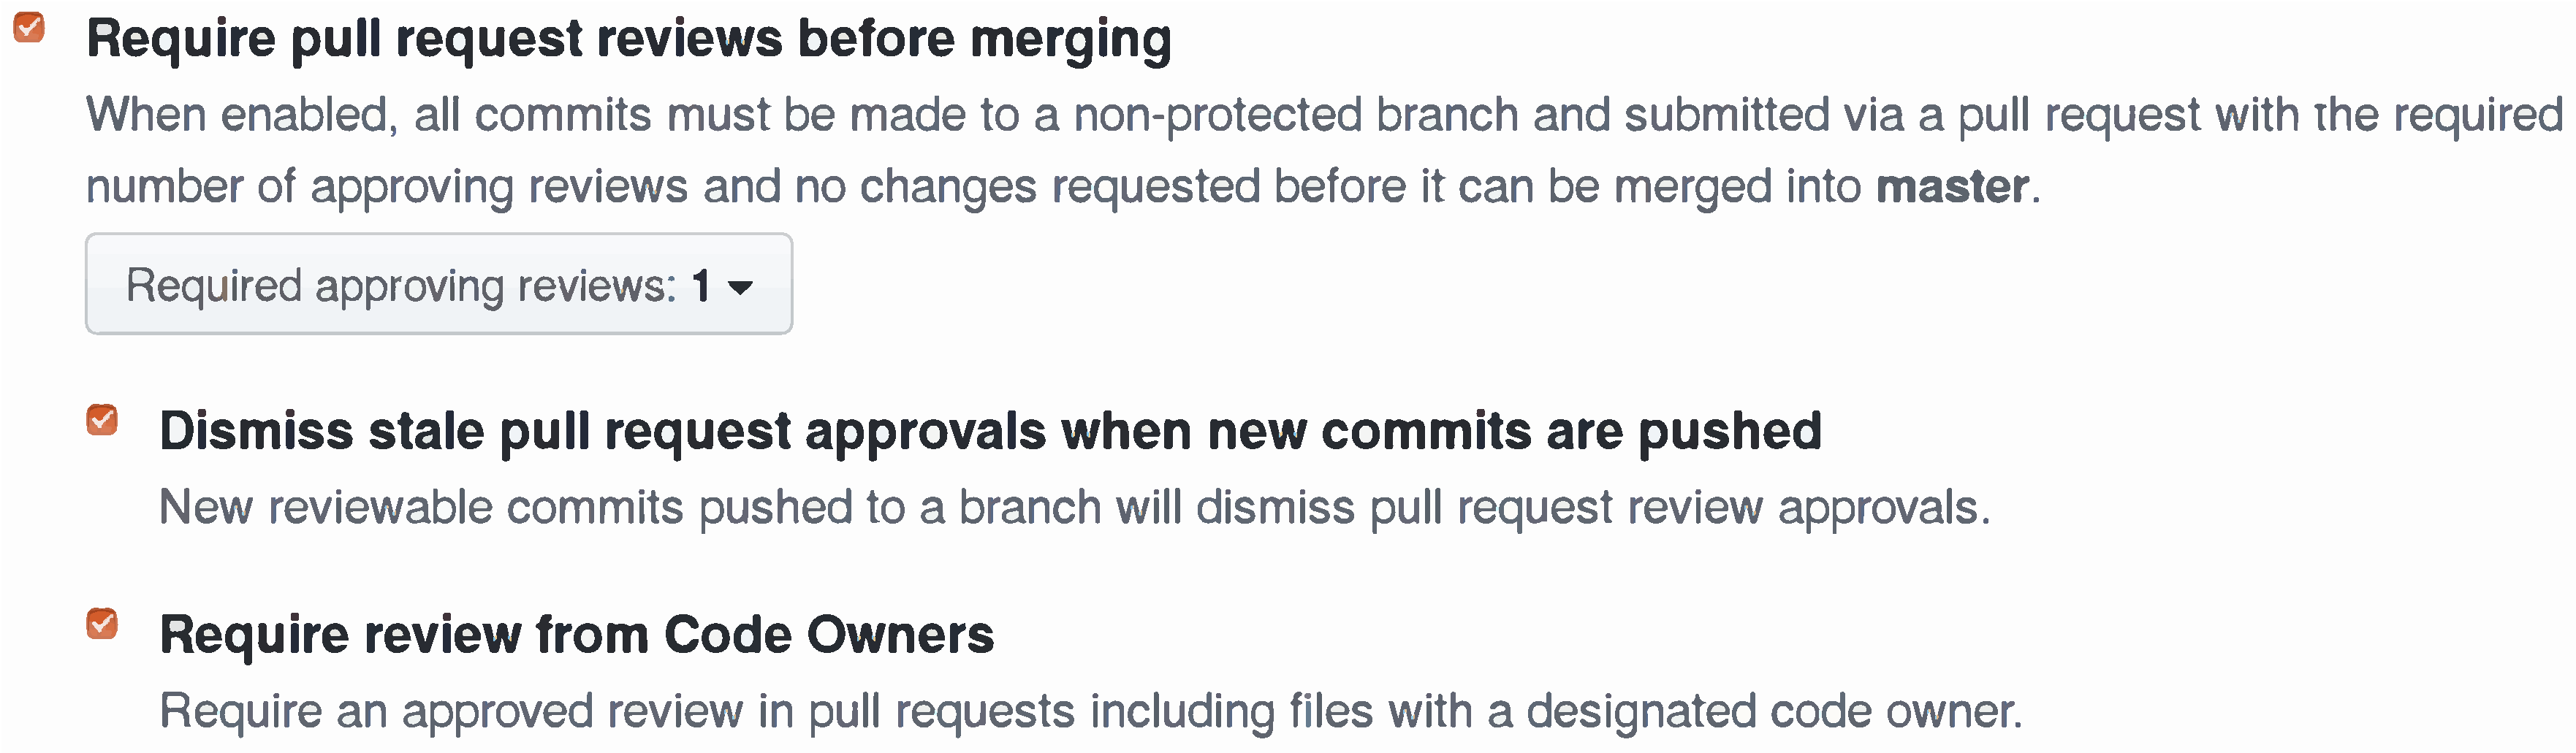
\includegraphics[scale=0.25]{img/codeowners_settings.pdf}
    \caption{Pull request reviews settings}
    \label{fig:codeowners_settings}
\end{figure}

The example in Figure~\ref{fig:codeowners_settings} shows the pull request reviews settings. The subsettings of \uv{\textit{Require pull request reviews before merging}} may not be set without \uv{\textit{Required approving reviews}} whose minimal value is one. The developers would like to be in possession with this helpful supplement of the development provided by the GitHub. Solution how to solve this problem resulted in a proposition which will enhance the bot - addition of a new feature to the bot which will keep the pull request mergeable.\\

During the implementation process of this task, GitHub unexpectedly adapted this feature as it was expected. Codeowners were requested for a pull request review automatically if the repository dispose of the codeowners file. These automated review requests were optional and they leave the pull request mergeable. The pull request\footnote{\url{https://github.com/ManageIQ/miq_bot/pull/417}} containing the unaccomplished implementation of that task was on this basis of premature refurbishment closed.

%=====================================================================================
\chapter{Conclusion}
%=====================================================================================

The goal of this thesis was to explain and bring you closer to the theoretical and technical background of the continuous integration and automated code review practices. Also, besides that, the thesis had an another aim which was successfully fulfilled - enhance the ManageIQ bot with new useful features that will make the development process easier. The enhancements of the bot were proposed on the basis of the continuous integration and automated code review analysis and the bot's problems and deficiencies which were discussed with the bot's maintainers. Some of the proposed enhancements were successfully integrated into the bot but some of them are currently under code review by the maintainers.\\

{\color{red}TODO - Jason's \& my summary}\\

This bachelor's thesis has been developed in collaboration with Red Hat, Inc. Thanks to this thesis, I have learned a lot about the method of how the open source projects are developed, how a group of developers works collaboratively worldwide and how open source project are enhanced by random contributors. I have acquired a lot of experiences about how to develop a software product together with others and how to contribute to other open source projects. Also, my imagination about my thesis has been met - I was working on something what will be useful and helpful for the future uses.
